\documentclass{llncs}

\usepackage{polyglossia}
\usepackage{todo}
\setmainlanguage{english}

%\usepackage{fontspec}
%\setmainfont{TeXGyreTermes}

\usepackage{url}

\title{Xodx}
\subtitle{a prove of concept and usability/practicability for the Distributed Semantic Social Network (DSSN)}
\author{}
\institute{\email{\{lastname\}@informatik.uni-leipzig.de}}

\begin{document}
\maketitle

\begin{abstract}
The Distributed Semantic Social Network is a new architecture for online social networks which has many benefits in terms of privacy, data security and data ownership.
The aim of this article is to examine if and how it is possible to setup a node of such a network on low cost and low powered hardware.
This report especially concentrates on the DSSN node implementation Xodx, its architecture and development.
\end{abstract}


\section{Introduction}
The World Wide Web (W3) is for long time not only a system for retrieving knowledge (Berners-Lee, 1992), but a interactive communication tool.
Online social networks have gained importance during the last years.
Currently the most used online social networks are facebook (1.1 bn), google plus (359 mio) and twitter (297 mio).
Compared to the absolute number of 2.7 billion W3 users approximately 40 \% of the W3 users are active on facebook.
This concentration on some services stays in contrast to the originally distributed nature of the W3 and the whole Internet as a network of decentralized organized computer nodes.

% Motivation
The current situation bears some risks regarding the privacy, data security, data ownership and reliability.
By building up a distributed online social network with multiple interlinked services those risks can be decreased.
The chose of the service a participant uses is completely up to her preferences.
On the one hand she can create an account at a big provider's service and doesn't has to care about the installation and maintenance of, on the other hand she can also go as far as setting up a personal service e.g. on a FreedomBox\footnote{see later, a freedom box is …} at home and keep the full control.
This topology is comparable to the distribution of e-mail-servers and has advantages regarding privacy, data security, data ownership, extensibility, reliability and freedom of communication (compare Tramp et al., 2012).
Every user is in the situation to control the availability and distribution of his own data without the need of being bound to the terms of service of a provider.

The aim of this paper is to prove that the concept of a DSSN as described in \cite{tramp-s-2012--a} is practically usable to run a social network.
For this purpose Xodx the implementation of a node for the DSSN, which provides the functionality needed for social communication in the Semantic Web is introduced in this paper.
- Setup testbed of multiple nodes to prove the interoperability


\section{The DSSN}
The Distributed Semantic Social Network (DSSN) is the idea of an architecture of an online social network, which consists of Linked Data RDF-Resources\footnote{See also Resource Description Framework (RDF) \cite{lassila-o-1999--a} and Linked Data \cite{bernerslee-t-2009--}} (from now on just called \emph{resources}), representing persons, which are placed on different nodes distributed across the Internet.
Thus each node holds a part of the network information and refers to other nodes.

As proposed in “An Architecture of a Distributed Semantic Social Network” \cite{tramp-s-2012--a} the DSSN is structured into four layers, the data, protocol, service and application layers.
The data layer contains the resources which can represent persons, applications, data- or media-artifacts and Atom-Feeds which are used to represent and publish temporarily ordered activities.
The protocol layer contains the WebID protocol for identification, Semantic Pingback \cite{tramp-s-2010--b} for proactive notifications to resources (e.g. befriending) and PubSubHubbub (PuSH) for resources to be subscribed to Atom-Feeds.
The service layer combines applications which have access for manipulation to the user's data. Until now the ping service, for receiving pings, the PuSH service, for publishing and subscribing to feeds, search and index services are defined.
Finally the application layer allows all different kinds of applications which the user gives access to, to access his data and act in his name.

A node in the DSSN has to understand (beside HTTP) the mentioned protocols (Semantic Pingback and PuSH).
It can provide data (resources and/or feeds and use-cases) about persons or artifacts in the data layer and/or provide services and applications on the service and application layers either only to the users of this node or also to other users of the DSSN.

\section{Xodx – a prove of concept and usability/practicability for the Distributed Semantic Social Network}
Because the DSSN should be optimally, from a privacy, data security and data ownership point of view, completely distributed across multiple nodes on the Internet the best would be to have one node per user where the user can control which data and services she wants to provide to others and which services he wants to use on other nodes.
The acceptance to run a personal node can be increased by minimizing the hardware requirements for the software and thus minimizing the costs for the users.
Xodx project\footnote{Xodx: \url{http://xodx.dssn.org}}, which is based on PHP.

\subsection{Requirements}
As argued in section (privacy, data security, data ownership, …) and in \cite{tramp-s-2012--a} for an online social network it is important to provide and support privacy, data security, data ownership and freedom of speech, which also presumes the reliability of the services.
An implementation of a node for the DSSN needs to provide to the user basic functionality for social communication. 
These basic functionalities are creating and editing a personal description, retrieve the personal descriptions of other persons, adding friendship relations, publishing status-messages, media-artifacts or arbitrary web-resources, subscribing to any web-resource's activity-feed (especially persons) and publish comments to those web-resources.

\subsection{Architecture}
Xodx is an implementation of the basic functionality of a DSSN node.
On the data layer it can be used for publishing resources and Activity-Feeds.
On the protocol and service layers it can receive Semantic Pingback-Pings and publish and subscribe to Atom-Feeds using PubSubHubbub (PuSH) .
Furthermore on the application layer it has a simple profile manager which can be used to create new person-resources and add new friendship-relations to it.
The architecture and intercommunication with other DSSN nodes and services is depicted in Fig. \ref{Xodx_arch}.

Xodx is constructed as a web application according to the model-view-controller (MVC) software design pattern which is supported by the Semantic Application Framework Saft\footnote{Semantic Application Framework Saft: \url{https://github.com/white-gecko/Saft}}.
PHP is used as programming language because Xodx makes highly use of the Erfurt Framework\footnote{Erfurt Framework: \url{http://erfurt-framework.org/}} and lib-dssn-php\footnote{lib-dssn-php: \url{https://github.com/AKSW/lib-dssn-php/}}.

\begin{figure}
    \begin{center}
        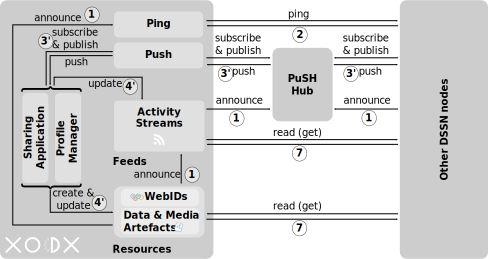
\includegraphics[width=.687\textwidth]{graphics/Xodx-in-DSSN-Architecture}
    \end{center}
\caption{The architecture of Xodx and its integration with other services and nodes}
\label{Xodx_arch}
\end{figure}


\subsection{Results}

\todo{funktionsumfang und vergleich mit Requirements section}

\section{Evaluation and simulation of semantic driven distributed social networks}
Because it is complicated to test the setup with real data retrieved from twitter due to copyright restrictions, we decided to create a framework which creates dummy samples.

- zweiter Hauptteil des papers
To evaluate the implementation we have designed an evaluation framework which simulates actions on the social network based on characteristics found on real social networks.
This framework can be adopted to any social network implementation and setup to be able to compare different systems.
We have also applied this framework to the DSSN run by distributed Xodx nodes.


\subsection{Evaluation Framework}
- aufbau von test copora (generierung und gathering)
- vokabular für simulation

The framework mainly consists of a simulation of the distributed network of nodes and the actual data generated by each node.
For this purpose we have designed a vocabulary which describes the setup of nodes with their accounts, the configuration of the nodes as well as the characteristics of each account.
Based on the account characteristics a corpus generator creates a file containing dummy-posts, which will be sent by the account.


We have found following characteristics necessary for our simulation:
the probability of creating original posts (narativity, in ppw – posts per week), the probability of responding to a received post or forwarding it (aka. retweet) (responsivity), the frequency of checking for incoming posts (updateprobability).
The amount of friendships (incoming/outgoing).

Based on \cite{zhao-d-2009--} we want to emulate heavy users with 626 to 1552 posts per 6 to 12 month (5 to 30 posts per week) and casual users with 48 to 167 tweets. They have 67 to 193 subscribers and 1 of 11 has 665 followers.

\subsection{Testbed}
- simulation (xodx)
We decided to simulate a completely distributed network where a new node is generated for every account.

\subsection{Results}


\subsection{Test Hardware and Software Environment}
The test hardware which was used for this practical is a Olimex A13-OLinuXino-WIFI board with an ARMv7 Cortex A8 processor at 1GHz (Allwinner A13 System on a chip), 512 MB RAM and 2–8 GB SD-Card-Storage.

The used operating system is a Debian GNU/Linux (arm hard float port, armhf) which was customized to boot and run on the board.
The kernel is a Linux 3.0.42 compiled from the sources provided by the Linux-Sunxi project\footnote{Linux-Sunxi project wiki: \url{http://linux-sunxi.org}, Kernel Sources: \url{https://github.com/linux-sunxi/linux-sunxi}}.

To get a web server environment the very light and resource efficient nginx was used to run PHP applications with the fast-cgi extension.
As database the Open\-Link Vir\-tu\-oso Open-Source Edition\footnote{Open\-Link Vir\-tu\-oso Open-Source: \url{http://ods.openlinksw.com/dataspace/doc/dav/wiki/Main/Main.VOSIndex}} was chosen because it is the best supported back-end for the Erfurt Framework.


\todos

\bibliographystyle{splncs03}
\bibliography{library}

\end{document}
